
% Podstawowe definicje dla wszystkich dokumentów

\documentclass[12pt]{mwart}
%\setlength{\textwidth}{83pt}

\usepackage[OT4,plmath]{polski}
\usepackage{amsmath,amssymb,amsfonts,amsthm,mathtools}
\usepackage{color}
\usepackage{fontspec}
\usepackage{listings,times}

\usepackage{bbm}
\usepackage[colorlinks=false]{hyperref}
\usepackage{url}
\usepackage{graphicx}

\graphicspath{{images/}}

\newcommand{\HRule}{\rule{\linewidth}{0.5mm}}

\newcommand{\term}[1]{
  \indent\textbf{#1}
  \vspace{5pt}
}

\usepackage{multicol}

\usepackage{capt-of}

\usepackage{lmodern} \normalfont
%\DeclareFontShape{EU1}{ptm}{bx}{n} { <-> ssub * cmr/bx/n }{}
%\DeclareFontShape{EU1}{ptm}{m}{sc} { <-> ssub * cmr/m/sc }{}

%\usepackage{fancyhdr}
%\pagestyle{fancy}
%\fancyhead{}
%\fancyhead[LE,LO]{Iron Coach. \doctitle}
%\fancyhead[RO,RE]{\rightmark}
%\fancyfoot{}
%\fancyfoot[LE,RO]{}
%\fancyfoot[CO,CE]{\thepage}
%\addtolength{\headheight}{1.5pt}

\widowpenalty=10000
\clubpenalty=10000
\linepenalty=1000
\hyphenpenalty=10000
\raggedbottom

\renewcommand{\labelitemi}{}
\renewcommand{\labelitemii}{}
\renewcommand{\labelitemiii}{}
\renewcommand{\labelitemiv}{}

\newcommand{\titlep}[2] {
  \newcommand{\doctitle}{#1}
  \thispagestyle{empty}
  \begin{titlepage}
    \begin{center}
      \textsc{Studencka Pracownia Baz Danych}\\[0.5cm]
      \textsc{\large Instytut Informatyki\\Uniwersytetu Wrocławskiego}\\[1.5cm]


      \vspace{3.5cm}

      % Author and supervisor
      \begin{minipage}{\textwidth}
        \begin{center} \large
          Łukasz \textsc{Czapliński}
        \end{center}
      \end{minipage}

      \vspace{0.5cm}



      % Title
      \HRule \\[0.4cm]
      { \Large Dokumentacja projektu \\[0.5cm] }
      { \Huge \bfseries Coffee Shop  \\[1cm] }

      \textsc{\Large #1\\\large Wersja #2}\\[0.5cm]

      \HRule \\[1.5cm]

      \vspace{1cm}

      
      \vfill
      

      \vspace{1cm}

      % Bottom of the page
      {\large Wrocław 2014}

    \end{center}
  \end{titlepage}
  \clearpage
  \setcounter{page}{2}
}

\newcommand{\chist}[1]{
  \begin{table}
  \centering
  \caption{Historia zmian}
  \begin{tabular}{l | l | p{5cm} | p{5cm}}
    Wersja & Data & Opis & Autor \\ 
    \hline
    \noalign{\smallskip}
    #1
  \end{tabular}
\end{table}
}


\begin{document}
\titlep{Dokumentacja ogólna}{1.0}
\chist{1.0 & 2014-06-13 & Powstanie dokumentu & Łukasz Czapliński\\
        }
\tableofcontents
\clearpage
\section{Wprowadzenie}
\subsection{Cel dokumentu}
Dokument ten ma na celu sprecyzowanie zadań projektu CoffeeShop i sposobów ich realizacji.
\section{Zadania projektu}
Celem projektu jest stworzenie aplikacji bazodanowej pozwalającej na obsługę prostego CoffeeShopu. Ma być on zdecentralizowany -- kilku właścicieli, z których każdy ma swoje towary. Mogą oni współdzielić dostawców towarów. Klienci mają mieć wybór co kupują od którego właściciela. 
Powinno się to odbywać zdalnie -- zarówno pomiędzy klientami a właścicielami (klient zamawia towary u konkretnego dostawcy, a ten kontaktuje się z nim w sprawie odbioru i zapłaty) oraz dostawcami i właścicielami (właściciel wybiera jaki typ produktu chce zamówić i kontaktuje się z dostawcą lub odwrotnie -- dostawca pyta właścicieli z którymi współpracował czego będą potrzebować).
\section{Model}
\subsection{Model konceptualny}
\begin{figure}
  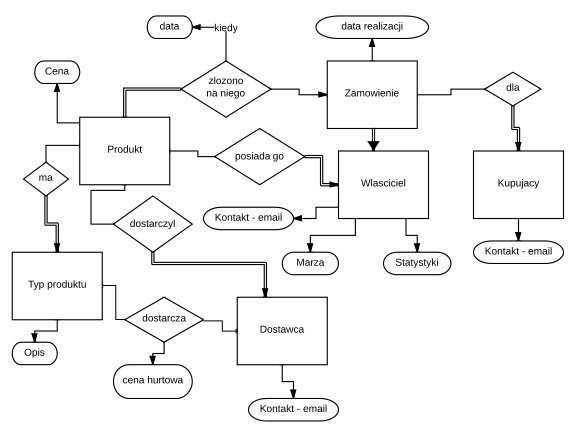
\includegraphics[width=0.99\textwidth]{model.png}
  \caption{Model konceptualny bazy danych}
  \label{konc}
\end{figure}
Jest przedstawiony na rys.~[\ref{konc}].\\
Można w nim wyróżnić 3 główne role: klient, dostawca i właściciel oraz 3 obiekty którymi operują: produkty, ich typy oraz zamówienia. \\
Klient składa zamówienia do właściciela na konkretne produkty.\\
Właściciel dodaje nowe produkty wybierając z oferty dostawców.\\
Dostawca rejestruje jakie typy produktów w jakiej cenie może zapewnić.\\
Zamawianie dostaw nie jest kontrolowane przez tą bazę danych -- odbywa się pomiędzy właścicielem a dostawcą przez umówione kontakty -- maile.
\subsection{Model fizyczny -- obiekty}
Każdy obiekt jest reprezentowany przez unikalny klucz -- liczbę nadawaną automatycznie z sekwencji oraz informacje dodatkowe. \\
\subsubsection{Dostawca i klient}
Osoby posiadają pole kontakt -- powinien być to mail (jest to automatycznie sprawdzane przy dodawaniu obiektu do bazy).
\lstinputlisting[language=SQL, firstline=46, lastline=50]{../../src/projekt.sql}
\lstinputlisting[language=SQL, firstline=13, lastline=18]{../../src/projekt.sql}
\subsubsection{Właściciel}
Dodaktowo wlaściciel ma określoną marżę -- wskaźnik ile procent sprzedawany przez niego produkt będzie droższy od jego ceny hurtowej.
\lstinputlisting[language=SQL, firstline=23, lastline=28]{../../src/projekt.sql}
\subsubsection{Typ produktu}
\lstinputlisting[language=SQL, firstline=4, lastline=9]{../../src/projekt.sql}
\subsubsection{Produkt}
Cena jest automatycznie wyliczaną wartością (na podstawie marży właściciela i ceny hurtowej): [\ref{prTrig}].
\lstinputlisting[language=SQL, firstline=55, lastline=63]{../../src/projekt.sql}
\subsubsection{Zamówienie}
Wartość zamówiona jest sumą cen produktów na niego się skłądających: [\ref{prTrig}].
\lstinputlisting[language=SQL, firstline=33, lastline=41]{../../src/projekt.sql}
\subsection{Model fizyczny -- związki dodatkowe}
\subsubsection{Kto dostarcza jaki typ produkt}
Tabela ta pozwala zapisać kto dostarcza jaki towar w jakiej cenie.
\lstinputlisting[language=SQL, firstline=67, lastline=72]{../../src/projekt.sql}
\subsection{Model fizyczny -- wyzwalacze}
\subsubsection{Aktualizacja ceny produktu i wartości zamówienia}
\label{prTrig}
Odbywa się po zmianie/dodaniu elementu do tabeli \textbf{produkt}.
\lstinputlisting[language=SQL, firstline=76, lastline=98]{../../src/projekt.sql}
\subsection{Model fizyczny -- role}
\subsubsection{Klient}
\lstinputlisting[language=SQL, firstline=203, lastline=209]{../../src/projekt.sql}
\subsubsection{Właściciel}
\lstinputlisting[language=SQL, firstline=193, lastline=200]{../../src/projekt.sql}
\subsubsection{Dostawca}
\lstinputlisting[language=SQL, firstline=211, lastline=218]{../../src/projekt.sql}
\end{document}
